\documentclass[authoryear]{elsarticle}
\usepackage[brazilian]{babel}
\usepackage[utf8]{inputenc}
\usepackage[T1]{fontenc}
\usepackage{lineno,hyperref}
\usepackage{float}
\modulolinenumbers[5]
\usepackage[authoryear]{natbib}
\journal{Journal of \LaTeX\ Templates}
\usepackage{graphicx}
%%%%%%%%%%%%%%%%%%%%%%%
%% Elsevier bibliography styles
%%%%%%%%%%%%%%%%%%%%%%%
%% To change the style, put a % in front of the second line of the current style and
%% remove the % from the second line of the style you would like to use.
%%%%%%%%%%%%%%%%%%%%%%%

%% Numbered
%\bibliographystyle{model1-num-names}

%% Numbered without titles
%\bibliographystyle{model1a-num-names}

%% Harvard
%\bibliographystyle{model2-names.bst}\biboptions{authoryear}

%% Vancouver numbered
%\usepackage{numcompress}\bibliographystyle{model3-num-names}

%% Vancouver name/year
%\usepackage{numcompress}\bibliographystyle{model4-names}\biboptions{authoryear}

%% APA style
%\bibliographystyle{model5-names}\biboptions{authoryear}

%% AMA style
%\usepackage{numcompress}\bibliographystyle{model6-num-names}

%% `Elsevier LaTeX' style
%%%%%%%%%%%%%%%%%%%%%%%
\bibliographystyle{elsarticle-num-names}
\begin{document}

\begin{frontmatter}

\title{An\'alise da base de dados abertos sobre gastos p\'ublicos da Prefeitura do Recife}


%% Group authors per affiliation:
\author{Allyson Manoel}
\author{Leonardo Alves}
\author{Marcos Barreto}

\begin{abstract}
Em uma prefeitura, cada gestão no comando possui um perfil próprio de direcionamento dos gastos públicos, uma análise histórica dos mandatos anteriores pode ser uma ferramenta de grande importância nas mãos dos cidadãos durante o período eleitoral. Tendo isso como base, o presente artigo busca traçar um comparativo da utilização dos recursos públicos entre os três últimos mandatos da Prefeitura do Recife (João Paulo Lima, João da Costa, Geraldo Júlio) compreendidos no período de 2005 à 2016.  
\end{abstract}

\begin{keyword}
\texttt{análise}\sep \texttt{dados}\sep \texttt{gastos} \sep \texttt{mandatos} \sep \texttt{Recife}
\MSC[2018] 62-07
\end{keyword}

\end{frontmatter}

\linenumbers

\section{Introdução}

O regime democrático brasileiro possui como base o voto popular, este é a principal ferramenta que o indivíduo possui de fazer valer os seus interesses individuais e coletivos. Buscar o melhor representante é uma tarefa complicada que exige conhecimento do perfil, histórico e propostas de cada candidato, aliado a isso, uma análise das gestões anteriores podem servir de indicativo de como políticos de mesmo partido irão atuar, uma vez que os mesmo são adeptos à sua corrente de pensamento\citep{adriana2013}. 

Como estudo de caso, no presente artigo será analisada a prefeitura do Recife, Pernambuco, especificamente no intervalo entre 2005 e 2016, período que compreende os mandatos de João Paulo Lima (PT), João da Costa (PT), Geraldo Júlio (PSB). Serão levantadas questões no que diz respeito aos investimentos em saúde, educação, mobilidade urbana e segurança, como foi a evolução dos investimentos ao longo dos meses e em período eleitoral, quais os setores mais beneficiados e quais foram os principais credores de cada gestão. 

Para a análise dos dados será utilizada a linguagem python e algumas de suas bibliotecas como pandas, para manipulação dos dados, HoloViews e Bokeh, para as visualizações dos dados. 
Inicialmente será apresentado o conjunto de dados utilizados utilizados e como foi realizado e as etapas de coleta o pré processamento. Posteriormente será feita uma análise comparativa de como cada gestão fez o direcionamento dos gastos públicos durante o mandato.

\section{Base de dados}
Nessa seção será discutido sobre a coleta e o pré-processamento da base de dados utilizada. Como também uma visão geral a respeito desses dados, e o que se pode inferir a partir deles.

\subsection{Coleta}

A etapa de coleta foi simples e direta. A Prefeitura do Recife disponibiliza publicamente as despesas realizadas pelo governo municipal com serviços, obras e compras. Essas informações são fornecidas pela Secretaria de Finanças, e são divididas por ano, de 2002 a 2018 até o momento, compreendendo assim três mandatos completos do período de 2005 a 2016, os quais foram selecionados para análise como objetivo desse projeto. Os arquivos estão no formato csv, facilitando assim seu acesso.

O sítio eletrônico onde se encontra essa base disponibiliza também o dicionário dos dados\citep{descricao2018}, ajudando no entendimento de cada atributo presente. 

\subsection{Pré-processamento}

Nessa etapa se fez necessário a compreensão de quais tipos de dados estão presentes no dataset, quais informações são mais relevantes para prosseguir para a etapa de análise, e que tipos de transformações deveriam ser realizadas.

A Prefeitura de São Paulo disponibiliza publicamente um documento, através da Secretaria do Tesouro, detalhando quase por completo os atributos presentes no dataset investigado\citep{transparenciasp2018}. Esse arquivo ajudou a entender o significado dos dados e a tomada de decisão para delimitar os atributos analisadas.

A partir dessa fase de pré-processamento, os datasets individuais de cada ano foram unificados em apenas um para facilitar o tratamento e análise dos dados. Primeiramente foi analisado a quantidade de valores nulos de cada atributo, encontrando números insignificantes, em comparação a magnitude da base, nos atributos: indicador de subempenho e os valores de empenho, liquidado e pago, o primeiro não foi considerado como relevante para a pesquisa por não trazer informações importantes para as hipóteses, e o restante não trazem prejuízos com seus valores nulos por eles representarem no máximo 0.005\%. Dessa forma, nenhuma medida de correção foi tomada para esses casos.


A base consiste em apenas dois tipos de atributos: nominal e numérico. Todos os atributos nominais, identificados pelo sufixo “\_nome”, vem acompanhado de um atributo numérico com sufixo “\_codigo”. Essa “tupla” representam a mesma informação, mas de forma diferente. Como os atributos nominais apresentam um teor informativo maior, por ser auto explicativo, todos os códigos foram removidos para simplificar o dataset.

Analisando mais profundamente alguns atributos nominais categóricos, foi notado que “unidade\_nome” apresentava categorias semelhantes, e aquelas que representavam a mesma informação foram unificadas, generalizando a informação, porém evitando perdas, ou simplificando, no momento da busca na etapa de análise.


O objetivo do projeto é focado nas despesas orçamentárias do governo municipal, e os atributos dos valores gastos são os principais na análise. Como eles representam a moeda real, é necessário uma transformação para que seja levado em consideração no cálculo a inflação, normalizando todos os valores para os dias atuais. Para esse processo, foi escolhido para base de cálculo o Índice Geral de Preços do Mercado (IGP-M) calculado mensalmente pela Fundação Getulio Vargas (FGV)\citep{fgvibre2018}. Esses números foram obtidos através da calculadora online disponibilizada pelo Banco Central do Brasil\citep{bcb2018}. A tabela 1 mostra os valores obtidos para correção, por ano.

\begin{table}[h]
\centering
\caption{Valor IGP-M anuais}
\begin{tabular}{r|lr}

Ano & Valor IGP-M \\ 
\hline                             
 2005 & 1.99 \\
 2006 & 1.94 \\
 2007 & 1.85 \\
 2008 & 1.69 \\
 2009 & 1.62 \\
 2010 & 1.56 \\
 2011 & 1.43 \\
 2012 & 1.35 \\
 2013 & 1.27 \\
 2014 & 1.21 \\
 2015 & 1.13 \\
 2016 & 1.04
\end{tabular}
\end{table}

Como os dados compreendem um período de 12 anos ao total, seria necessário a correção de 144 meses. Como forma de simplificação, foi tomada a decisão de obter apenas um valor IGP-M por ano, considerando apenas as correções dos meses de janeiro e dezembro de cada ano em questão, e sendo calculado a média aritmética desses valores, estabelecendo um valor único por ano.

Devido a diversos fatores externos em relação à economia do país, cada mandato administra quantidades distintas de verbas. Assim, seria injusto comparar os mandatos pela quantidade real de dinheiro destinada aos diferentes setores. Dessa forma os valores empenhados, liquidados e pagos contidos na base de dados foram normalizados para a porcentagem em relação ao total gasto, por mandato. Ou seja, para cada um dos três mandatos foram calculados a quantia total das despesas orçamentárias, e para cada uma das despesas ao longo dos quatro anos de cada mandato, os três valores mencionados foram normalizados de acordo com seus respectivos totais.

\section{Análise}
Nessa seção será discutido sobre a discussão e seleção dos atributos escolhidos para a análise, assim como a forma que os dados foram separados e por fim a discussão e os resultados da análise exploratória sobre os dados coletados.

\subsection{Seleção de atributos}

Após o pré-processamento, a base de dados apresenta vinte e quatro atributos. Apenas cinco deles são numéricos, sendo o ano e mês da movimentação orçamentária, e os valores empenhado, liquidado e pago. Todos esses foram considerados essenciais. Os demais são atributos categóricos nominais. Dentre os dezenove disponíveis, apenas quatro foram utilizados: unidade orçamentária, função, grupo de despesa e credor.

Em unidades orçamentárias encontra-se diversas secretarias, alguns fundos e gabinetes municipais. Em função, de acordo com[3], caracteriza o maior nível de agregação das diversas áreas de atuação do setor público, relacionando com a missão institucional do órgão,  como por exemplo, cultura, educação e saúde. Grupo de despesa é um agregador de elementos de despesa com as mesmas características quanto ao objeto de gasto, como por exemplo pessoal e encargos sociais, investimentos e amortização de dívida. E por fim, o credo é a pessoa física ou jurídica que está sendo pago pelo município ao serviço solicitado.

Esses atributos mencionados foram considerados mais relevantes, e consequentemente, utilizados na etapa da análise exploratória.


\subsection{Separação de dados}
Para melhor manipulação dos dados e análise comparativa, a base de dados foi subdividida em três partes, cada uma correspondendo ao período de cada mandato: 2005 a 2008, 2009 a 2012 e 2013 a 2016.
\subsection{Análise exploratória}

Para iniciar a análise exploratória com foco em comparar os mandatos, é necessário obter uma visão geral da quantidade de recurso financeiro utilizado pelas gestões. Como explicado anteriormente, é vital esse primeiro contato com os valores reais pagos, para se ter uma noção dos perfis dos gestores, uma vez que o estudo comparativo será feito por meio da porcentagem utilizada.
\graphicspath{{figuras/}}
\begin{figure}[H]
\centering
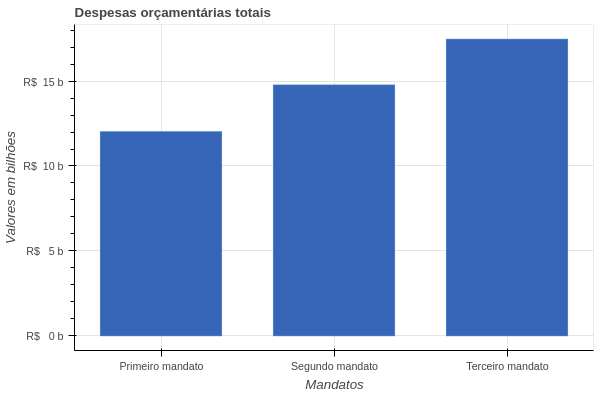
\includegraphics[scale=0.5]{figura_1.png}
\caption{Despesas orçamentárias totais}
\label{Rotulo}
\end{figure}
A figura 1 apresenta essa visão geral. Claramente cada prefeito administrou quantias diferentes da verba destinada ao município durante seu mandato, com uma diferença média de 3 bilhões de reais.
\graphicspath{{figuras/}}
\begin{figure}[H]
\centering
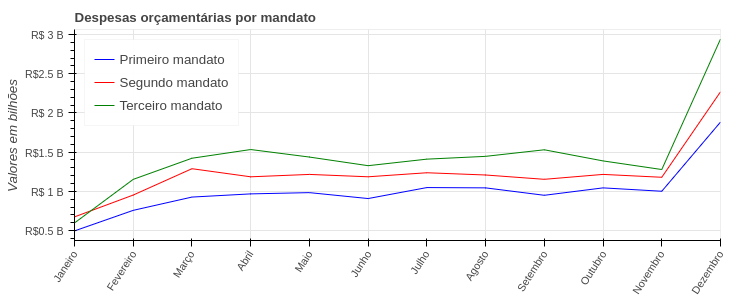
\includegraphics[scale=0.5]{figura_6.png}
\caption{Despesas orçamentárias totais}
\label{Rotulo}
\end{figure}

A figura 2 descreve um perfil aproximado de gastos durante cada mandato, agrupados por mês. Iniciando cada ano com poucos gastos, aumentando gradativamente até meados de abril, que a partir daí segue uma linearidade, finalizando com uma leve queda em novembro, mas encerra o ano com um aumento brusco. Posteriormente esse comportamento novembro-dezembro será analisado e discutido.

Dado a visão geral da quantidade de gastos em cada gestão, e o perfil mensal, pode ser questionado sobre qual o comportamento quanto aos setores básicos para com os cidadãos e a cidade: saúde, educação, mobilidade urbana e segurança. A figura 3 e 4 mostram que os três mandatos apresentam perfis similares quanto ao dinheiro destinado à saúde e a mobilidade urbana. O segundo prefeito representa bem a média, entre 22\% a 23\% para saúde e 10\% para mobilidade, e o terceiro superando com uma pequena margem.

\graphicspath{{figuras/}}
\begin{figure}[H]
\centering
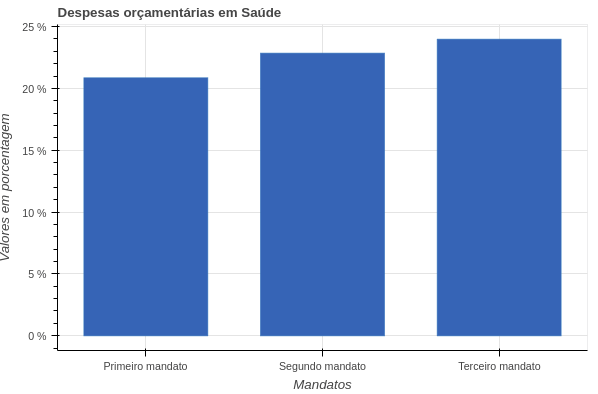
\includegraphics[scale=0.5]{figura_7.png}
\caption{Despesas orçamentárias totais}
\label{Rotulo}
\end{figure}


\graphicspath{{figuras/}}
\begin{figure}[H]
\centering
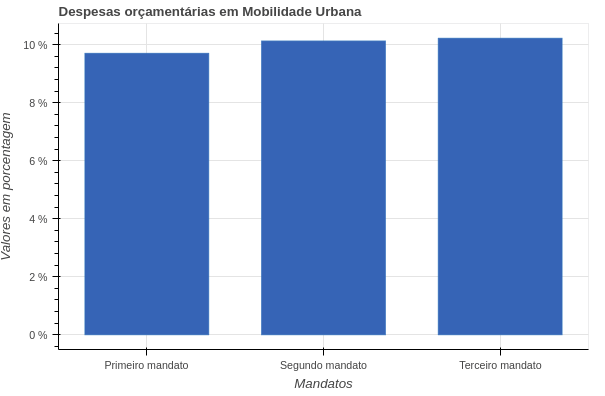
\includegraphics[scale=0.5]{figura_9.png}
\caption{Despesas orçamentárias totais}
\label{Rotulo}
\end{figure}

Para a educação o cenário muda levemente, porém agora o primeiro mandato toma a “liderança” com uma margem de 3\% superior aos demais, ressaltando que educação e saúde somam um pouco mais de 40\% de “investimento” total.


\graphicspath{{figuras/}}
\begin{figure}[H]
\centering
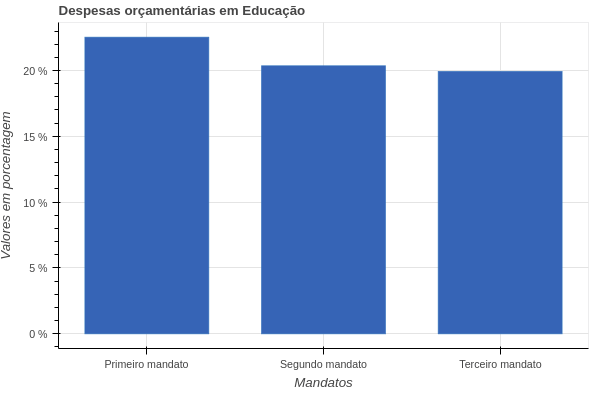
\includegraphics[scale=0.5]{figura_8.png}
\caption{Despesas orçamentárias totais}
\label{Rotulo}
\end{figure}

Por fim, o caso mais alarmante, o maior “investimento” em segurança pública entre os três mandatos foi apenas 2\%. A figura 6 ilustra essa informação.

\graphicspath{{figuras/}}
\begin{figure}[H]
\centering
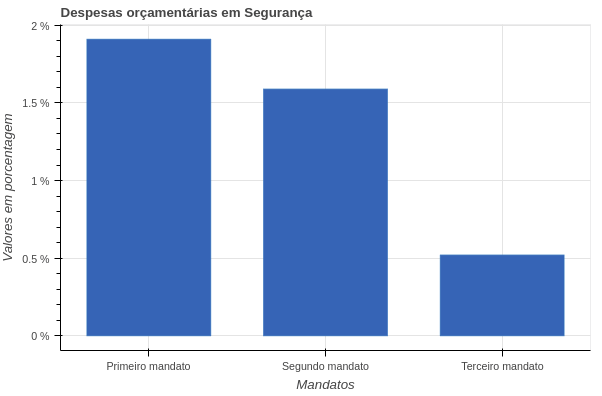
\includegraphics[scale=0.5]{figura_10.png}
\caption{Despesas orçamentárias totais}
\label{Rotulo}
\end{figure}

\section{Conclusão}

\section*{References}

\bibliography{mybibfile}

\end{document}